\documentclass[a4paper,11pt]{article}

\usepackage[plain]{fullpage}
\usepackage{graphicx}  %This enables the inclusion of pdf graphic files in figures
\usepackage{wrapfig}
\usepackage[utf8]{inputenc} %For "spesielle" tegn som æ, ø, å og andre er det anbefalt å angi dette. Mac brukere kan vurdere applemac og ikke utf8
\usepackage[norsk]{babel} %Inkluder kun dersom du vil skrive rapporten på norsk. Dette gir riktig datoformat og sørger for andre lokaliseringsting.
\usepackage[hidelinks]{hyperref}
\usepackage{pdfpages}
\usepackage{float}

\title{TDT4180 MMI: Øving D2}
\author{Gruppe 18: \\ Øyvin Richardsen, Sandor Zeestraten, Stian Habbestad, Rune Bjønnum, Kristian Våge}
\date{\today}
 
\begin{document}
\maketitle

\tableofcontents

\newpage

\section{Beskrivelse av brukergrensesnitt}
\subsection{Innledning}
Vi har valgt å bruke digitale mockups i stedet for papirprototyper. For å lage mockupsene brukte vi nettapplikasjonen \emph{Moqups} \cite{moqups}. For å knytte sammen mockupsene til en interaktiv prototype brukte vi \emph{InVision} \cite{invision}. Den finnes forøvrig her \cite{invisio}. 

\subsection{Deler av brukergrensesnittet}
\subsubsection{Loginvindu}
Loginvinduet er det første som brukeren møter når han starter kalenderapplikasjonen. Vinduet består av to tekstfelter for brukernavn og passord. Så to knapper for å logge inn samt glemt passord. Vi har valgt å ikke gå inn på grensesnittet for \emph{glemt passord}. Dersom brukernavn og passordet stemmer på serveren etter at brukeren har trykket på \emph{Login} så vil vinduet lukkes mens hovedvinduet åpnes. Hvis det ikke stemmer så vil brukeren få beskjed om hva som var galt.

\begin{figure}[H]
\centering
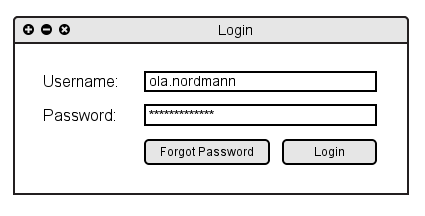
\includegraphics[scale=0.65]{images/login.png}
\caption{Loginvindu}
\label{login_image}
\end{figure}

\subsubsection{Hovedvindu}
Hovedvinduet har oversikten over avtalene i en uke-visning og en liste over notifikasjonene som berører brukeren (avtaler som har blitt endret eller kansellert). Forskjellige visninger som arbeidsdager, enkle dager, månedvisningen samt klokkeslett på venstresiden er ikke tatt med her. Det er tre forskjellige knapper, \emph{ny avtale}, \emph{flere kalendere} og \emph{logg ut}. \emph{Ny avtale} og \emph{flere kalendere} bringer opp nye vindu, mens \emph{logg ut} logger ut brukeren, lukker vinduet og bringer tilbake loginvinduet.

\begin{figure}[H]
\centering
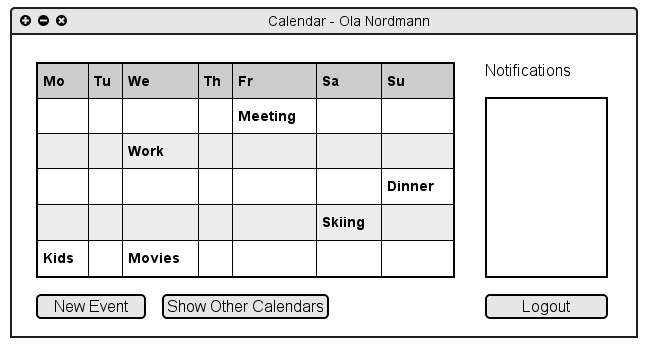
\includegraphics[scale=0.65]{images/hovedvindu.png}
\caption{Hovedvindu}
\label{hovedvindu_image}
\end{figure}

\subsubsection{Avtaleviser}
hello

\begin{figure}[H]
\centering
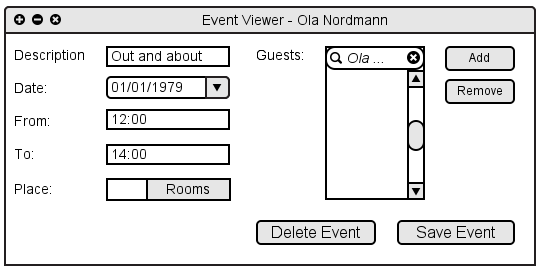
\includegraphics[scale=0.65]{images/avtaleviser.png}
\caption{Avtaleviser}
\label{avtaleviser_image}
\end{figure}

\subsubsection{Romreservasjon}
hello

\begin{figure}[H]
\centering
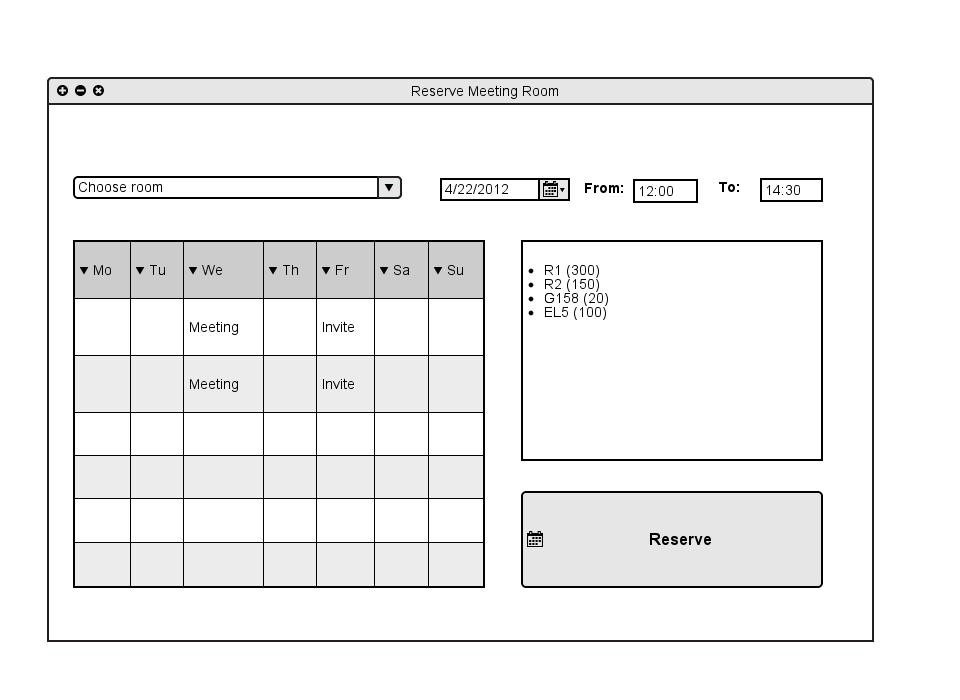
\includegraphics[scale=0.65]{images/romreservasjon.png}
\caption{Romreservasjon}
\label{romreservasjon_image}
\end{figure}

\subsubsection{Flere kalendere}
hello

\begin{figure}[H]
\centering
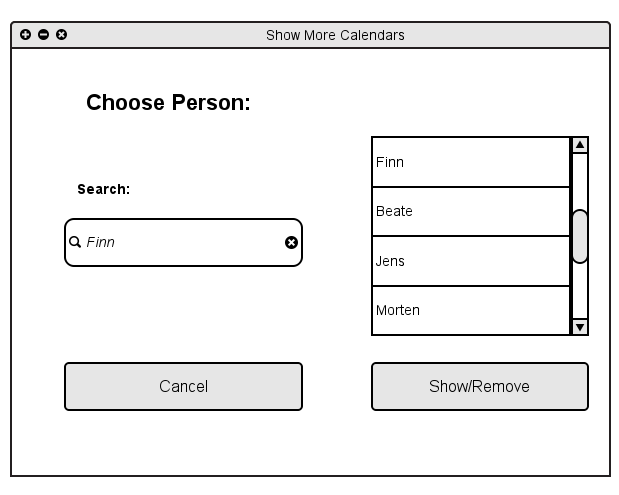
\includegraphics[scale=0.5]{images/flerekalendere.png}
\caption{Flerekalendere}
\label{flerekalendere_image}
\end{figure}

\subsubsection{Notifikasjon}
hello

\begin{figure}[H]
\centering
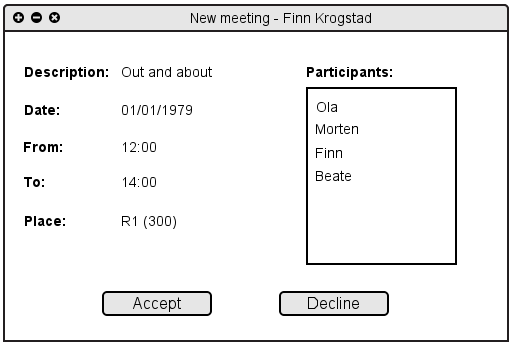
\includegraphics[scale=0.65]{images/notifikasjon_akseptert.png}
\caption{Notifikasjon akseptert}
\label{notifikasjon_akseptert_image}
\end{figure}

\begin{figure}[H]
\centering
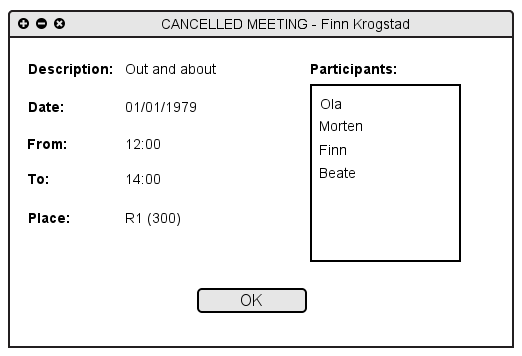
\includegraphics[scale=0.65]{images/notifikasjon_kanselert.png}
\caption{Notifikasjon kanselert}
\label{notifikasjon_kanselert_image}
\end{figure}


\subsection{Tilstandsdiagram}
Tilstandsdiagram

\begin{figure}[H]
\centering
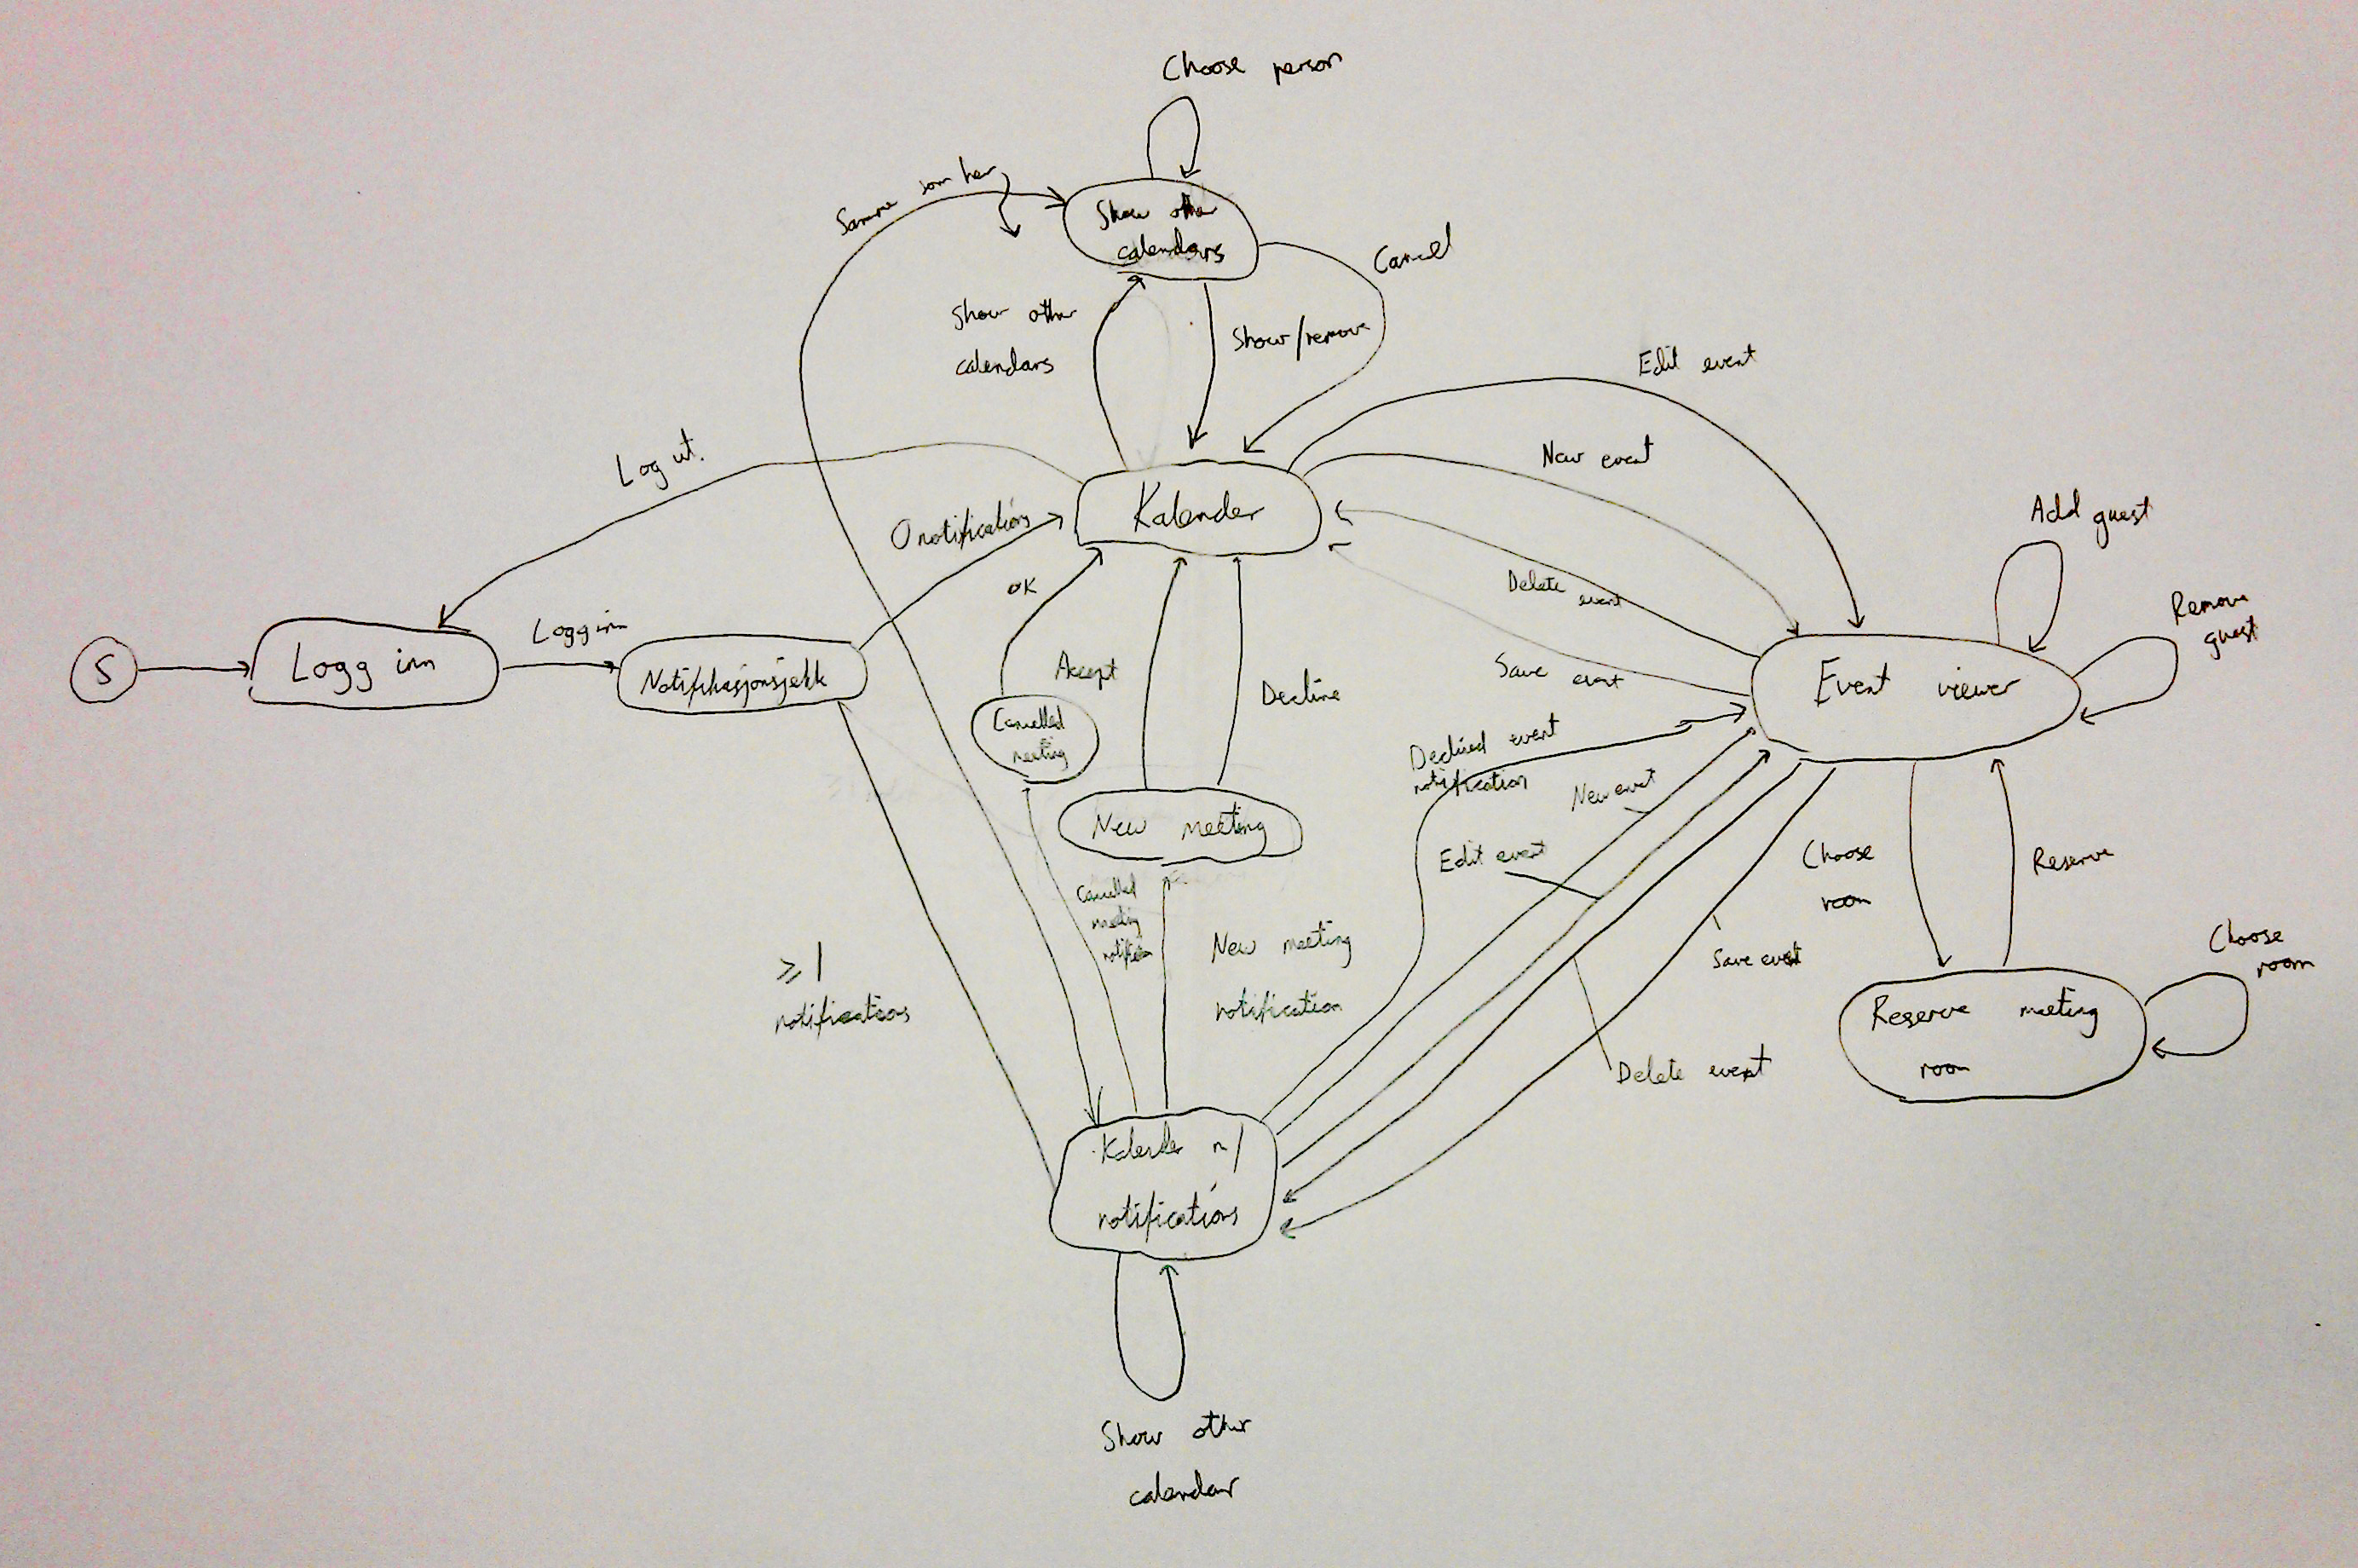
\includegraphics[scale=0.165]{images/tilstandsdiagram.jpg}
\caption{Tilstandsdiagram}
\label{tilstandsdiagram_image}
\end{figure}

\section{Beskrivelse av oppgavene og scenariene}
Hver testperson fikk utlevert et oppgavesett som skulle løses ved hjelp av vår prototype, se vedlegg: \hyperlink{vedlegg/cases.pdf.1}{\underline{Cases}}. Settet bestod av seks ulike case, der hvert case var satt sammen av en rekke punkter, som skulle gjennomgås i gitt rekkefølge av testpersonen, uten innblanding fra testleder og observatører. Dette for å kartlegge i hvilken grad brukergrensesnittet var intuitivt nok til å kunne brukes uten veiledning.

\subsection{Case 1}
	I første case skulle testpersonen logge seg inn på kalendersystemet som Ola Nordmann, og legge inn en ny avtale. Tre deltakere, kalt Beate, Morten og Finn, skulle inviteres, og møterom R1 skulle reserveres.

\subsection{Case 2}
	Formålet med andre case var å sjekke om testpersonen forsto varslingssystemet i kalenderapplikasjonen. Testpersonen skulle logge inn som Finn Krogstad, som ble invitert til møtet fra første case, og avslå alle nye avtaler. Testpersonen måtte selv finne ut hvordan varsel om nye avtaler er implementert i prototypen.

\subsection{Case 3}
	I tredje case ble testpersonen, etter å ha logget inn som Ola Nordmann, møtt av et varsel om at Finn Krogstad hadde avslått møteinnkallelsen. Tidspunkt for møtet skulle derfor endres til senere på dagen. Deretter skulle testpersonen logge inn som Finn Krogstad, og sjekke at det var kommet ny innkalling med oppdatert tidspunkt. Målet med testen var at testpersonen skulle prøve å redigere en avtale, og sjekke at eventuelle gjester fikk beskjed om endringene.

\subsection{Case 4}
	Fjerde case startet på samme måte som tredje case. Her skulle testpersonen ta bort Finn fra møteinvitasjonen. Finn Krogstad skulle få beskjed om at møtet var avlyst, noe testpersonen skulle bekrefte.

\subsection{Case 5}
	I femte case skulle testpersonen, logget inn som Ola Nordmann, prøve å avlyse et møte. Testpersonen skulle så bekrefte at Finn Krogstad hadde fått beskjed om at møtet var avlyst.

\subsection{Case 6}
	Sjette case skulle teste funksjonaliteten for å vise andre brukeres kalender sammen med sin egen. Testpersonen, logget inn som Ola Nordmann, skulle først prøve å vise kalenderen til Beate, og bekrefte at hennes avtaler ble vist sammen med Ola sine. Deretter skulle Beates kalender skjules.

\section{Hvordan ble testen gjennomført?}
Vi kjørte to iterasjoner på testen, med to ulike testere. I fra den andre gruppen var det Merete og så Ove som testet. I 

den første iterasjonen var Kristian leder, Stian og Øyvin var testobservatører. I den andre iterasjonen var Stian leder og 

Øyvin testobservatør. Kristian og Rune ble testet av den andre gruppen. 

Testen ble gjennomført ved at vi hilset på testeren og introduserte oss kort. Deretter gikk vi i gang med å forklare 

hvordan testen skulle utføres. Vi hadde også laget oss et lite manus som vi benyttet. (Appendix)



\section{Resultat fra brukbarhetstesten}
Målet med brukbarhetstesten er å finne områder der brukeren ikke forstår hvordan
han skal komme seg videre i programflyten, og se at brukeren klarer å finne
den informasjonen han ønsker.

Etter testen ga vi dem et SUS-skjema - System Usability Scale. Dette lar
brukeren gi tilbakemelding i form av poeng fra 1-5 på skalaen sterkt enig til
sterkt uenig. Testen er delt opp i likt antall negativt og positivt ladde
spørsmål. Disse spørsmålene er vevd sammen annenhver, men i teksten nedenfor
kaller jeg positive spørsmål del1 og negative del2 siden disse summeres hver for
seg. Del1 = spørsmål 1,3,5,7 og 9 og del2 = 2,4,6,8,10.

Hos Merete scoret vi 4+3+4+4+2 = 17 på del1 og 2+3+1+3+4 = 13 på
del2. Hos Ove scoret vi 3+2+3+3+3 = 14 på del1 og 4+4+3+3+4 = 18 på
del2. Dette ga score (17+13) * 2.5 = 75 for Merete og (14+18) * 2.5 = 80
fra Ove. De to scorene ble altså 75/100 fra Merete og 80/100 fra Ove. Dette gir
et snitt på 77.5/100.

Det er litt interessant og observere at Merete ga høyest poeng på de positivt
ladde spørsmålene, mens Ove ga mest poeng på de negativt ladde spørsmålene.

Mye av den tilbakemeldingen vi fikk etter testen tydet på at det som var mest
uklart var flyten gjennom de forskjellige casene. Det var litt forvirrende når
både case 4 og 5 var avhengige av at case 1 og 2 ble gjort om igjen. Vi burde
nok ha fokusert på å lage mer frittstående caser, slik at vi bedre kunne testet
flyten i programmet, og ikke i casene.

En score på 77.5 er ikke spesielt bra, men jeg tror en del av minuspoengene kom
fra litt forvirrende scenarier, og at de hadde litt høyere forventninger når
papirprotypene våre var interaktive og på pcen. I forhold til den gruppen som
vi testet sammen med, så var det morsomt når de la frem masse informasjon i
et klikk, mens når vi la inn masse informasjon når en hoppet til neste bilde, så
virket det kanskje litt forvirrende.

\begin{figure}[obs]
\centering
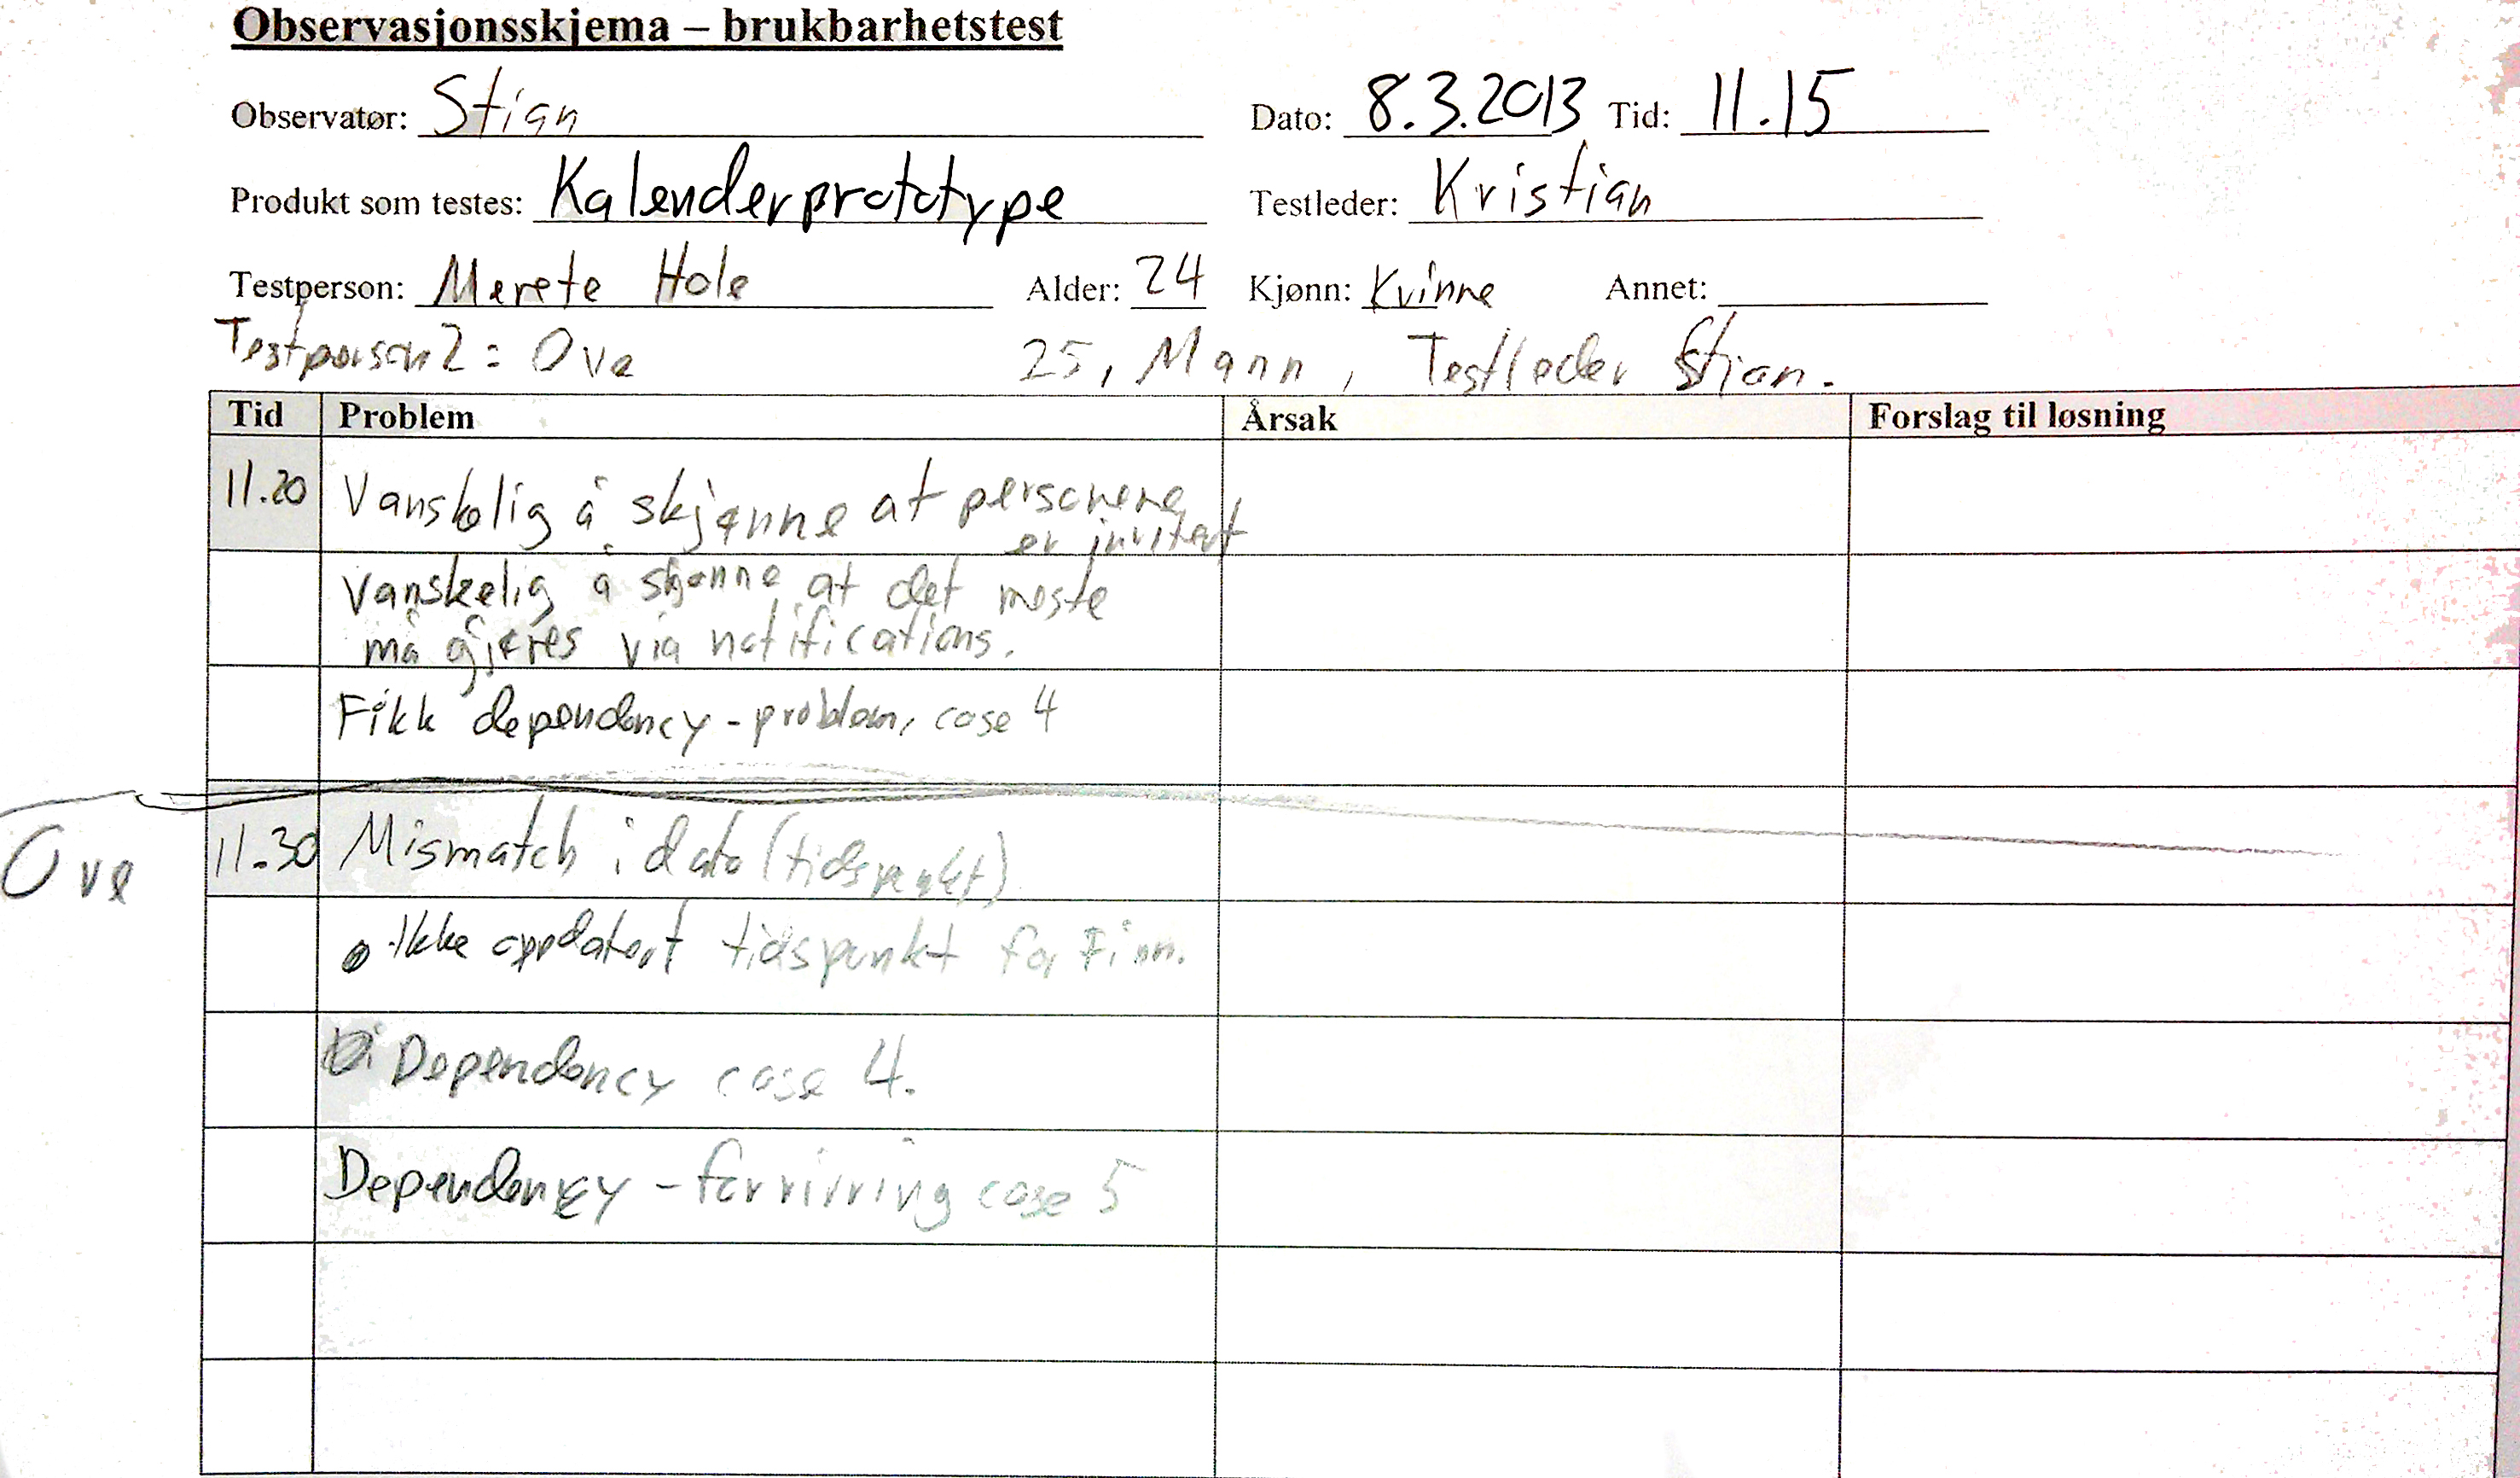
\includegraphics[width=160mm]{images/observasjon.jpg}
\caption{Observasjon}
\label{overflow}
\end{figure}

\begin{figure}[mer]
\centering
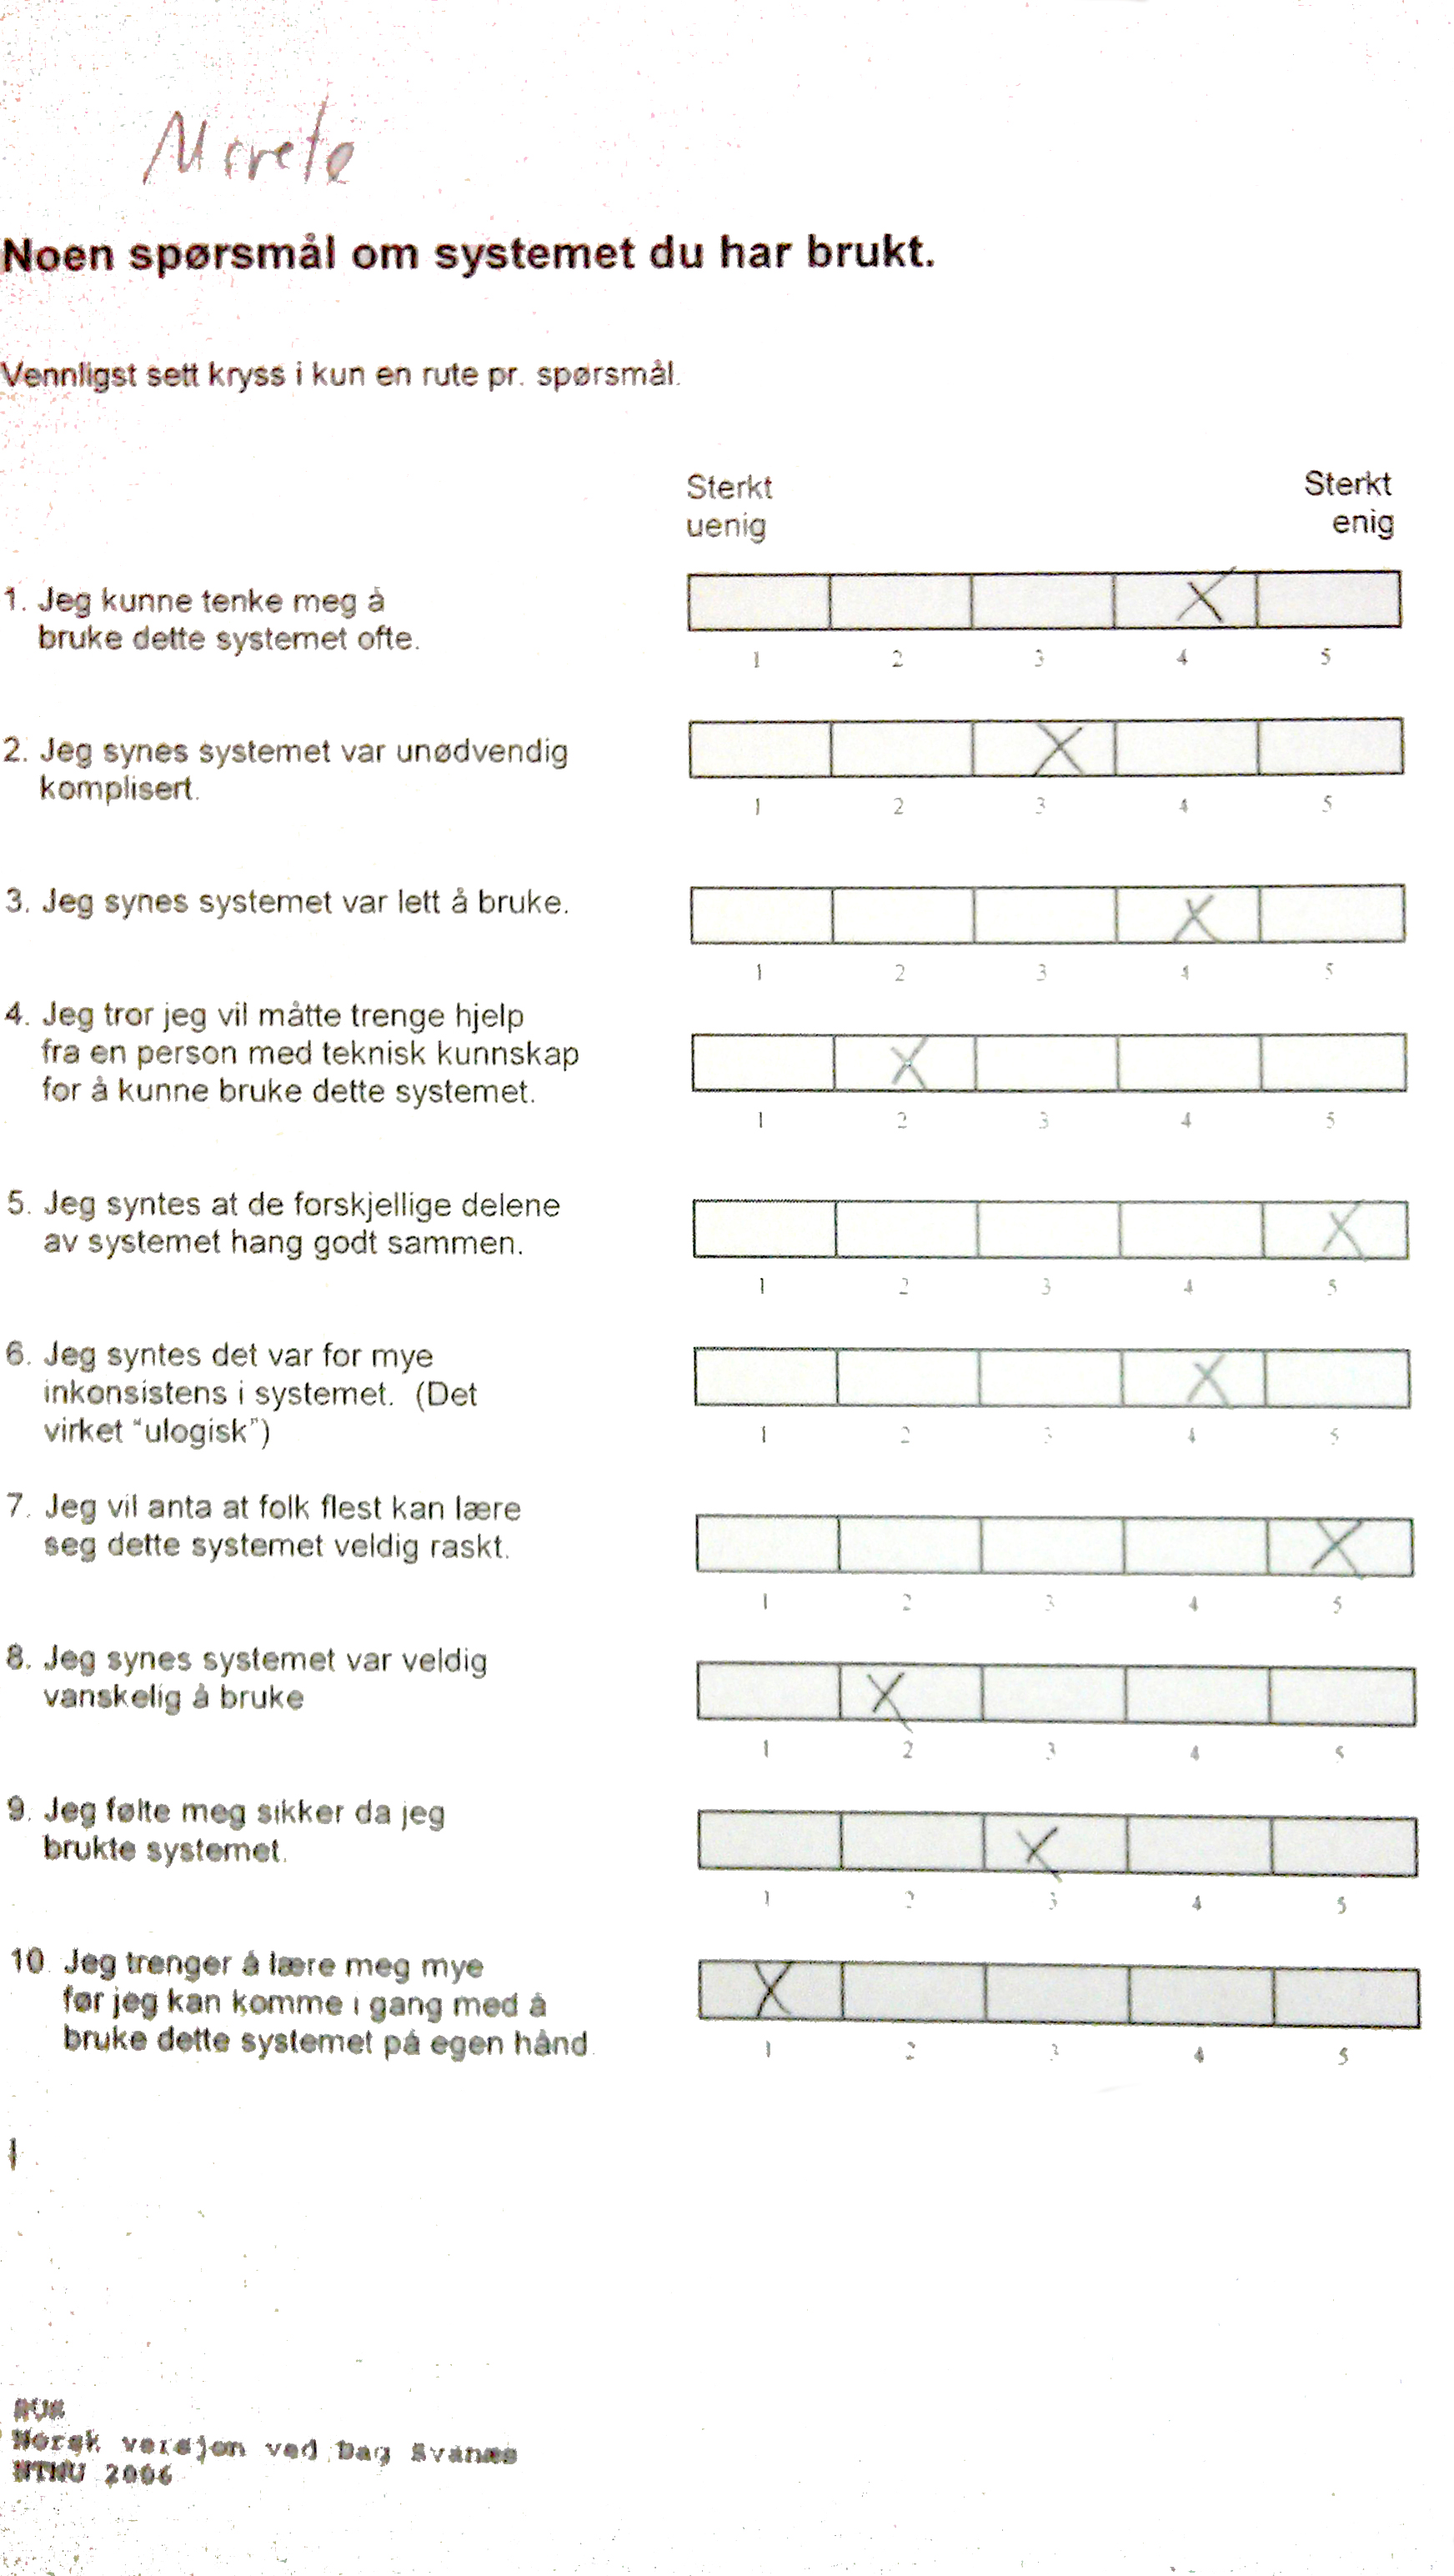
\includegraphics[width=140mm]{images/tilbakemelding_merete.jpg}
\caption{Tilbakemelding fra Merete}
\label{overflow}
\end{figure}

\begin{figure}[ove]
\centering
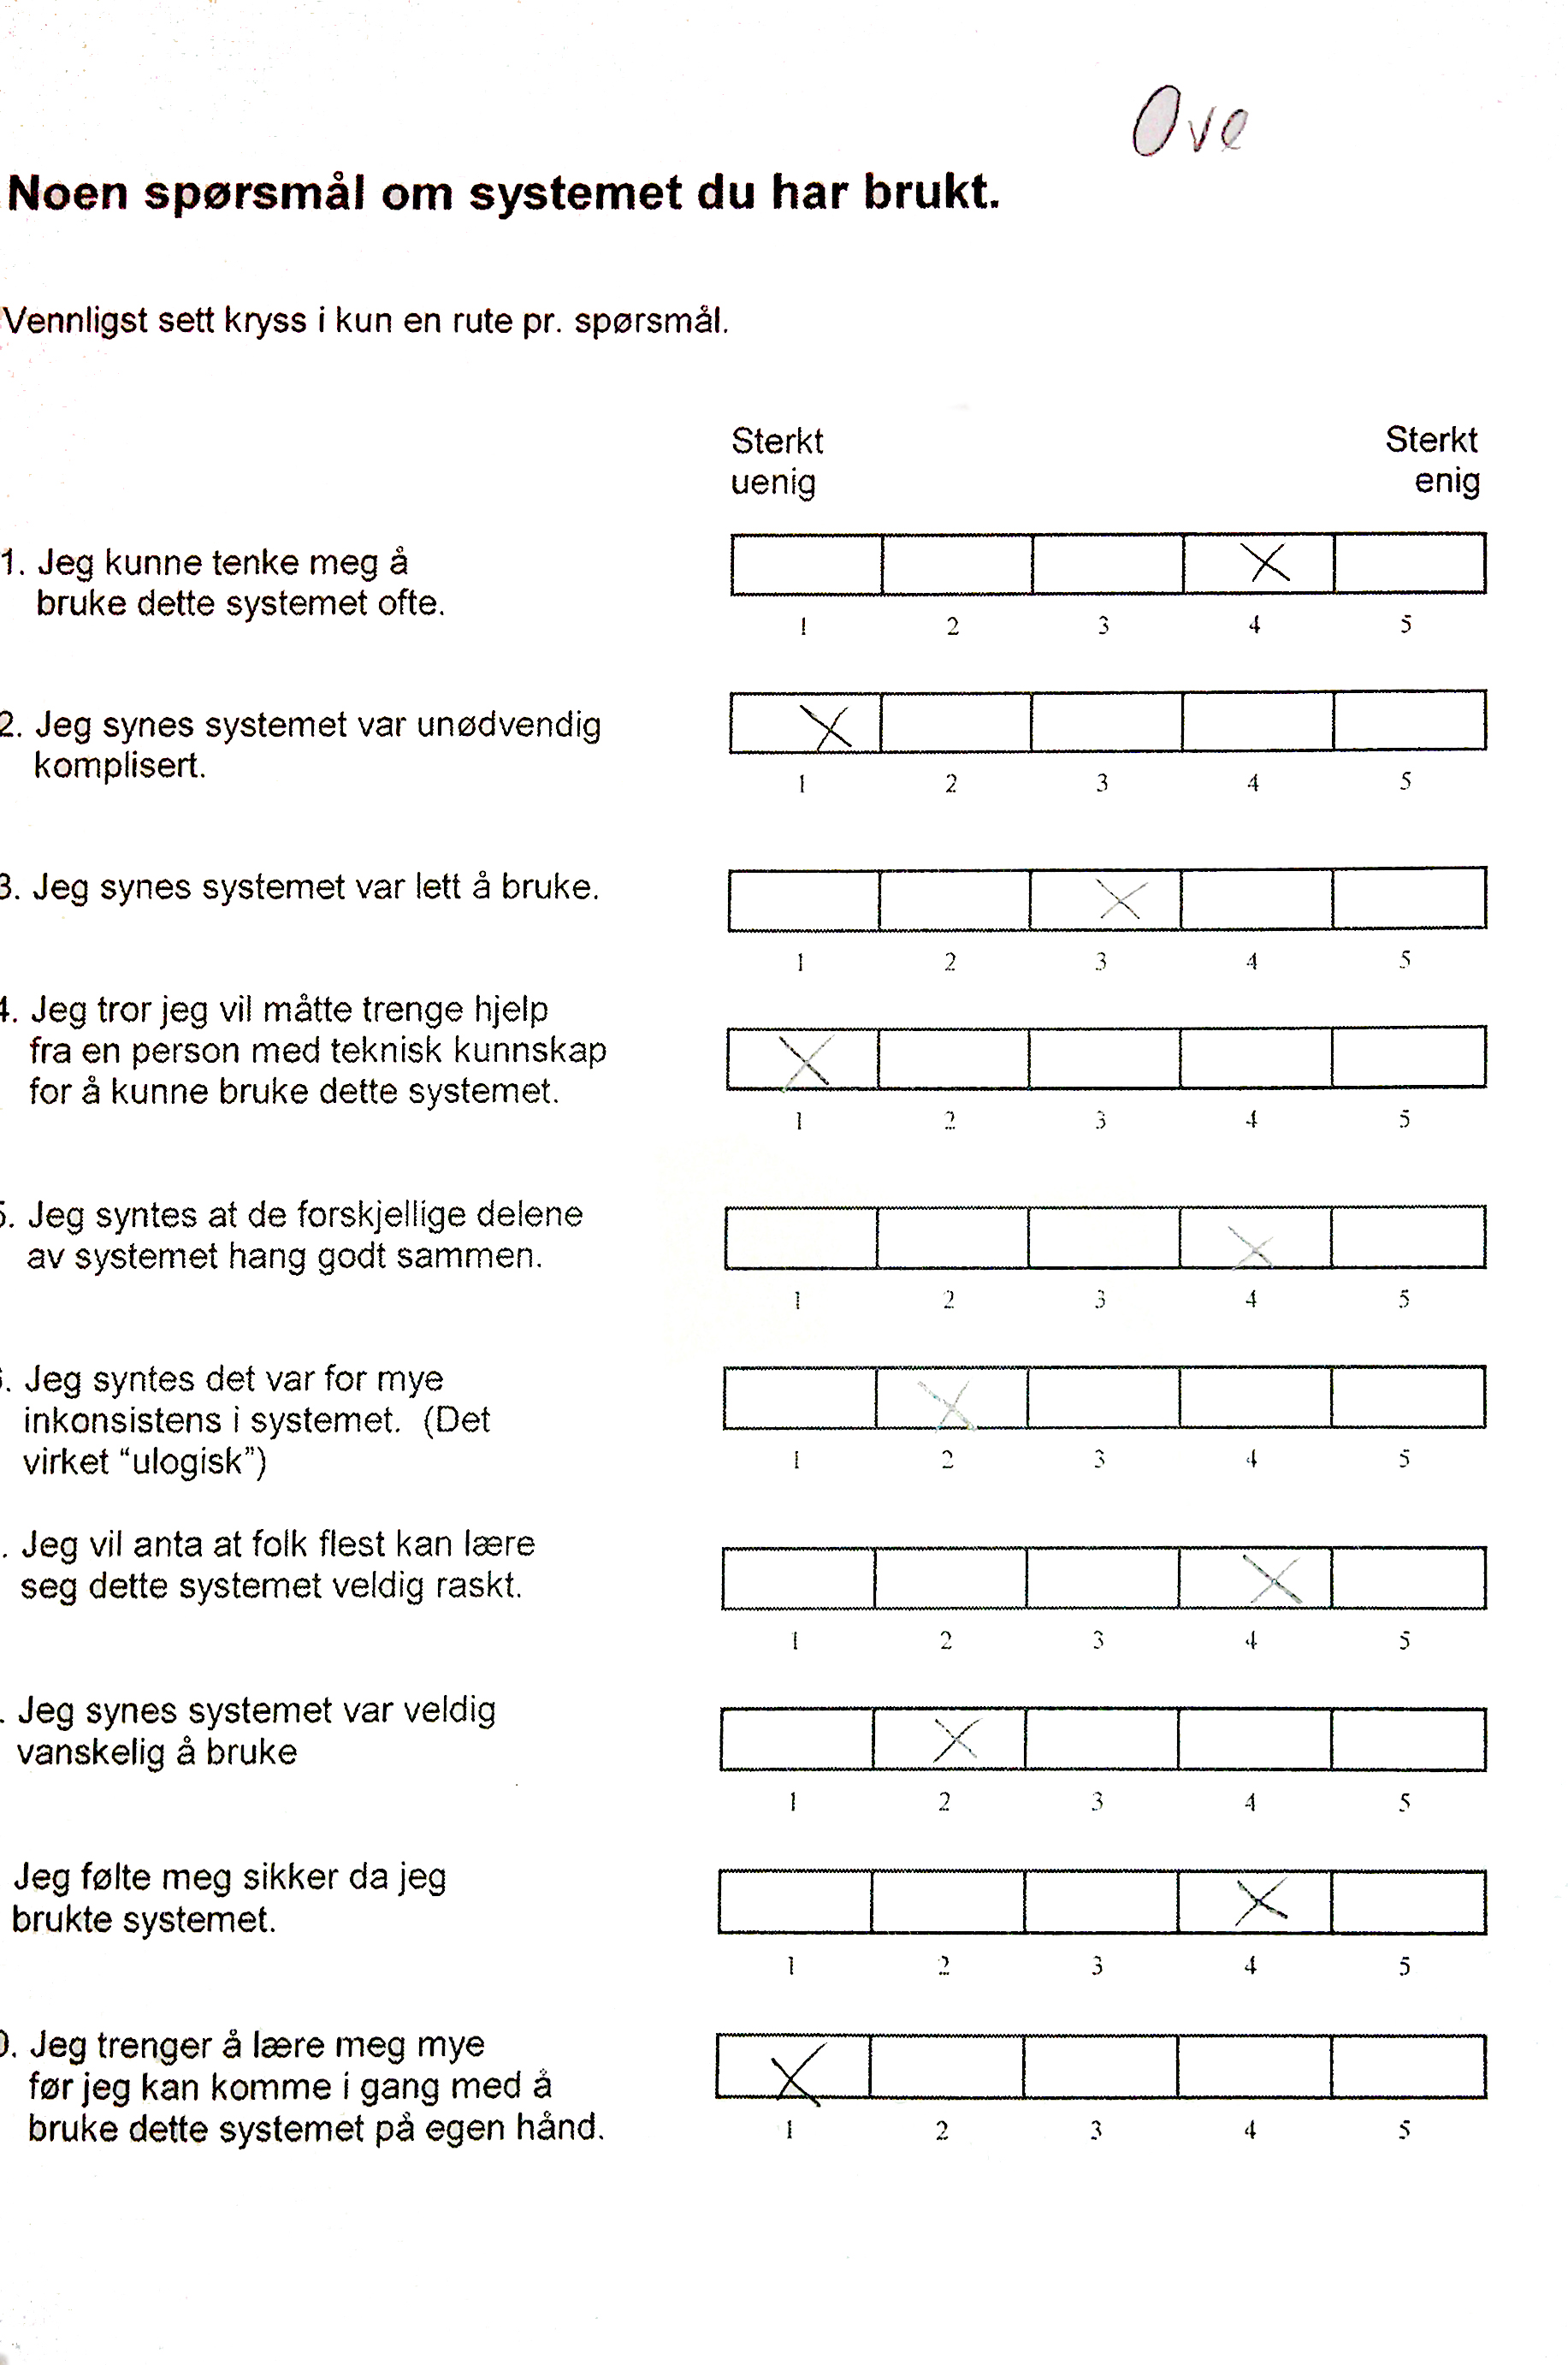
\includegraphics[width=140mm]{images/tilbakemelding_ove.jpg}
\caption{Tibakemelding fra Ove}
\label{overflow}
\end{figure}


\section{Forslag til redesign}
Basert på tilbakemeldinger

\footnotesize{  % This makes the Reference items print in footnotesize fonts
\begin{thebibliography}{N}
\bibitem{moqups} Moqups - Nettapplikasjon for mockups og prototyper \url{http://moqups.com}
\bibitem{invision} InVision - Interaktive prototyper \url{http://invisionapp.com}
\bibitem{invisio} Vår InVision prototype på nett \url{http://invis.io/CHCG09KM}

\end{thebibliography}.  
}


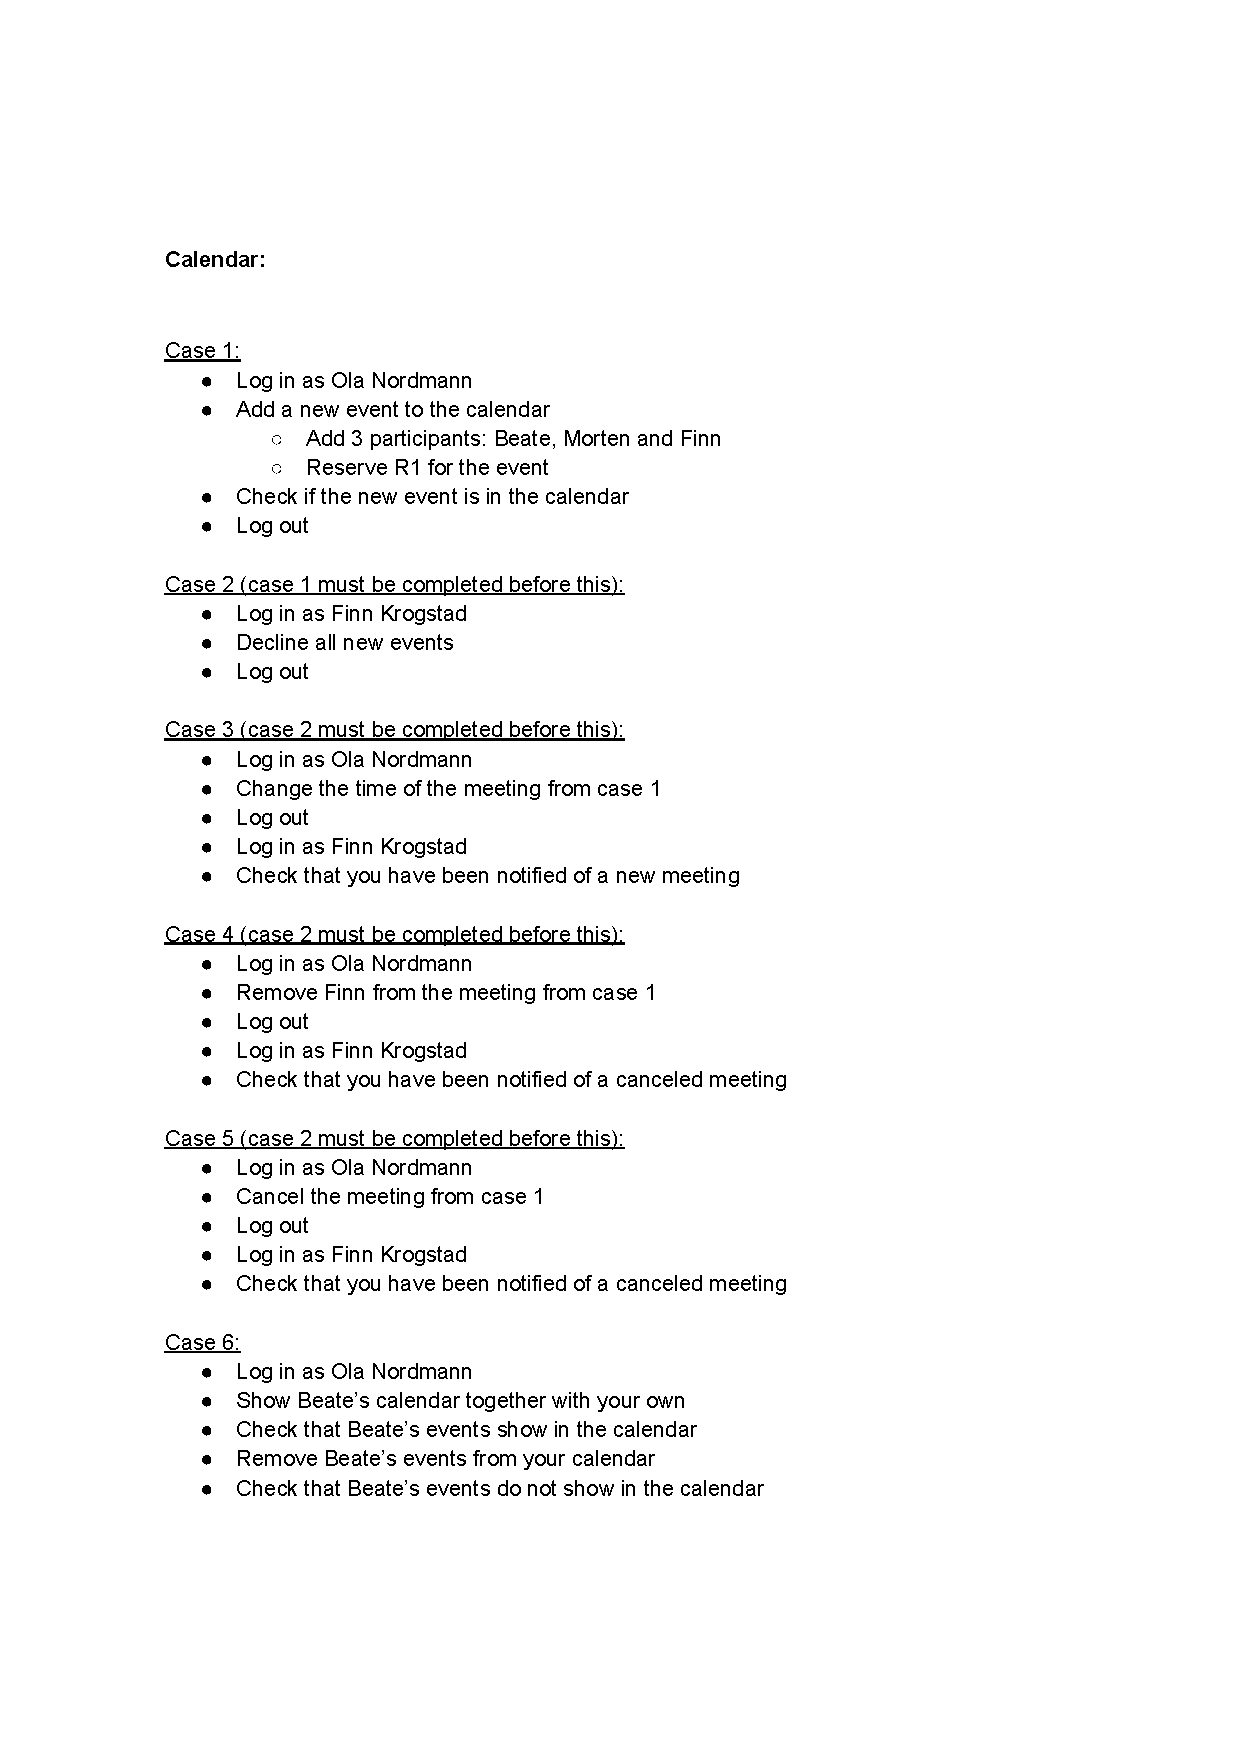
\includepdf[link,pages={1}]{vedlegg/cases.pdf}
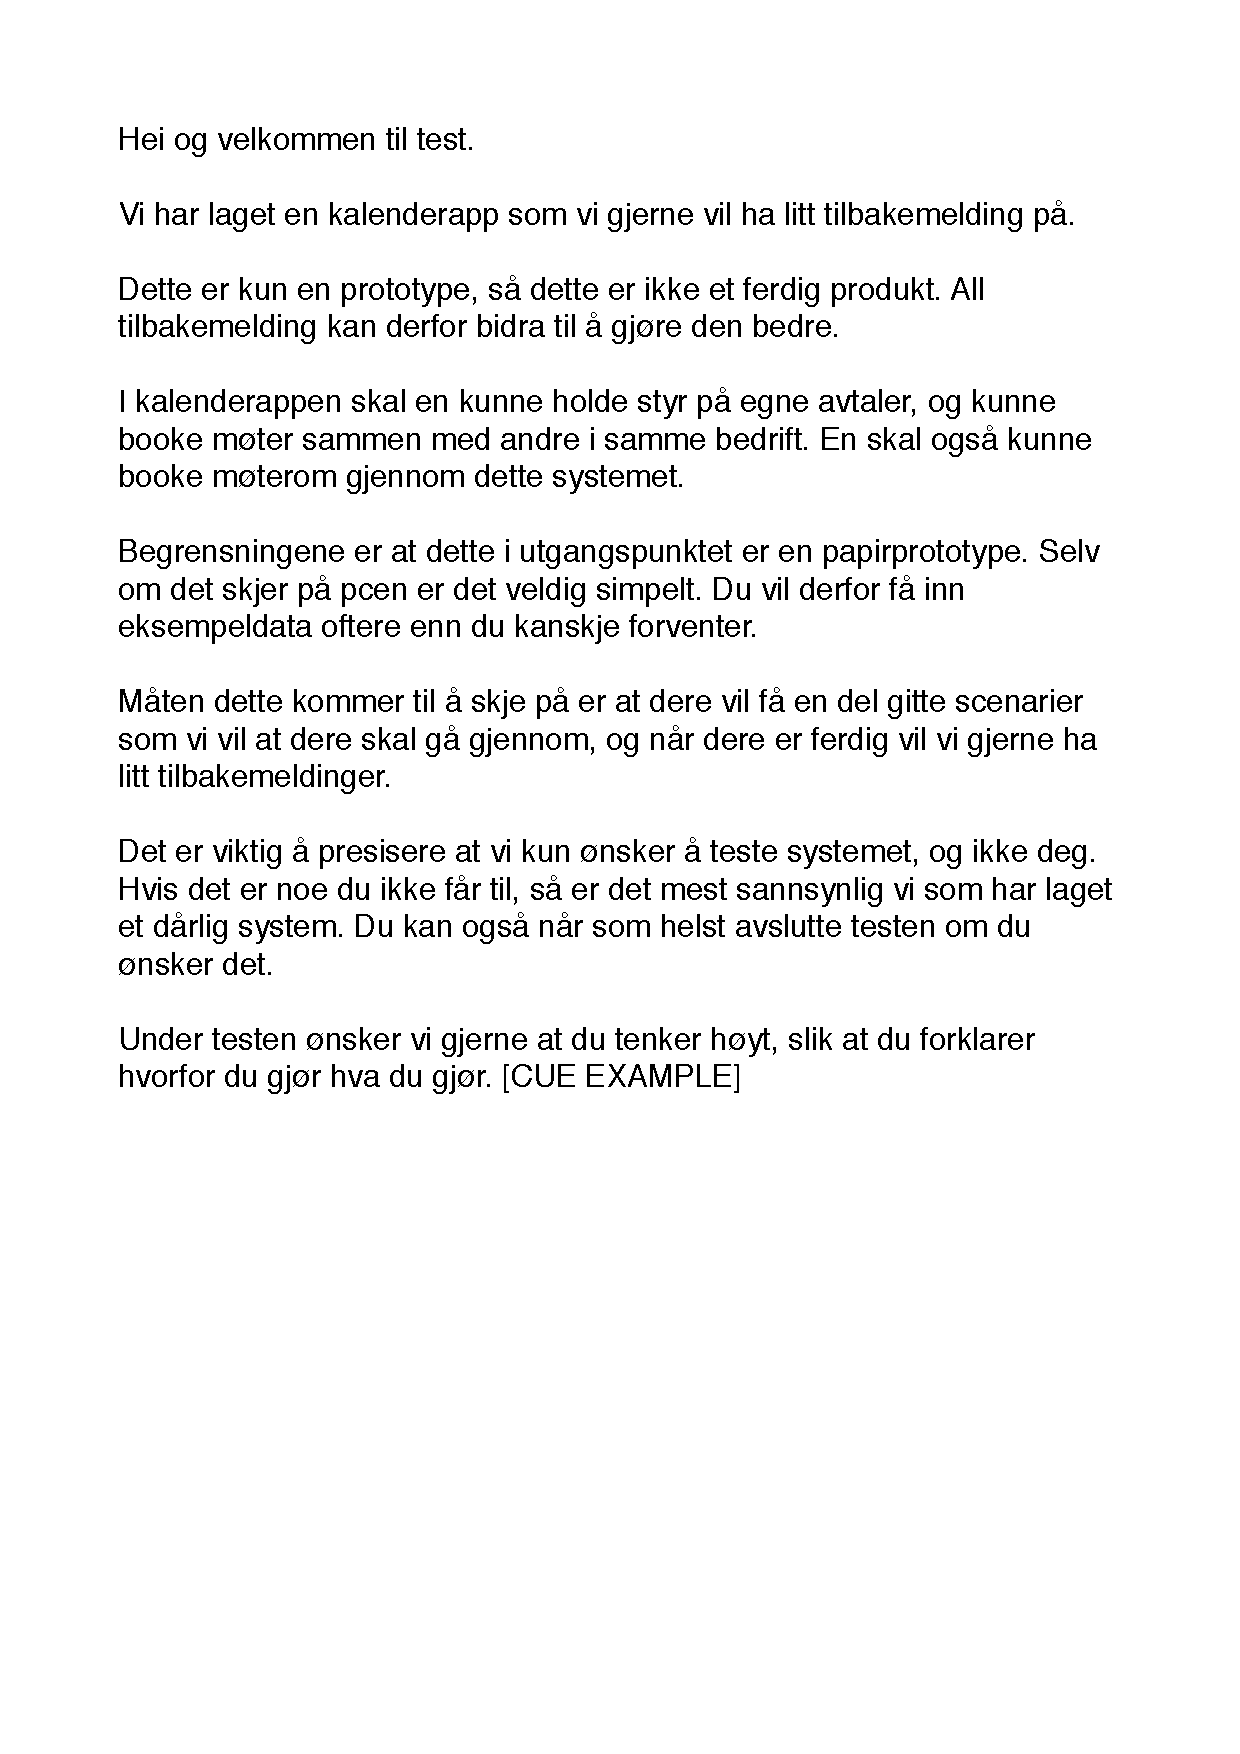
\includepdf[pages={1}]{vedlegg/manus.pdf}

\end{document} 